\documentclass[11pt]{article}

\usepackage[left=1in,right=1in,top=0.7in,bottom=0.75in]{geometry}
\usepackage[T1]{fontenc}
\usepackage{lmodern}
\usepackage{amsmath,amssymb}
\usepackage{booktabs}
\usepackage{graphicx}
\usepackage{float}
\graphicspath{{figures/}{report/figures/}}
\usepackage{xcolor}
\usepackage[colorlinks=true,linkcolor=blue!50!black,citecolor=magenta,urlcolor=blue!50!black]{hyperref}
\usepackage[labelfont=bf]{caption}
\renewcommand{\figurename}{Fig.}
\setlength{\intextsep}{8pt plus 2pt minus 2pt}
\setlength{\abovecaptionskip}{4pt}
\renewenvironment{abstract}{%
  \par\small\begin{quote}%
  \noindent\textbf{Abstract.}\enspace\ignorespaces
}{\end{quote}}
\makeatletter
\def\@openbib@code{%
  \advance\leftmargin\bibindent
  \itemindent-\bibindent
  \listparindent\itemindent
  \itemsep 2pt\relax
  \parsep\z@}
\makeatother

\newcommand{\R}{\mathbb{R}}
\newcommand{\dB}{\,\mathrm{dB}}

\title{What Determines the Effectiveness of 3D Field of Junctions?\\
{\large A Study of Volumetric Denoising Applications}}
\author{Samudraneel Sarkar, Sakshi Patil$^{*}$, Nikhil Kumar$^{*}$,
Manpreet Singh$^{*}$\\[1.4em]
MNNIT Allahabad\\[0.2em]
{\small\texttt{\{samudraneel.20233249, patil.20233209, nikhil.20233202,
manpreet.20233180\}@mnnit.ac.in}}}
\date{}

\begin{document}
\maketitle
\begingroup\renewcommand{\thefootnote}{}%
\footnotetext{$^{*}$Equal contribution; order determined by coin flip.}%
\endgroup
\vspace{-2em}

\begin{abstract}
3D Field of Junctions (FoJ) is a training-free denoiser that fits each
patch of a volume with planar wedges meeting at a common vertex and
averages the overlapping fits. Its demonstrated applications are
low-dose X-ray CT, cryo-electron tomography, and point-cloud denoising.
We apply 3D FoJ to three domains outside that set, porous-media
micro-CT, an MRI phantom, and binary porous media, and compare it with
Gaussian, median, and total-variation (TV) filtering across noise
levels to examine when the method helps and when it fails. At its
default configuration, the method reduces to an independent wedge fit
per patch followed by averaging, with no inter-patch coupling. From
this mechanism follow three requirements for FoJ to help. First, the
input must be unbiased: each region intensity is a mean of the voxels
it covers, so a systematic offset in the input is reproduced rather
than removed. Second, the structure must be piecewise-flat at or above
the patch scale; features smaller than the patch cannot be represented
by wedges, and the output collapses toward the mean. Third, the input
noise must be high enough that the wedge model's bias is paid for by
the noise it removes.
\end{abstract}

%=====================================================================
\section{Introduction}

Volumetric images acquired under dose and time limits are noisy, and
denoising is a routine step in their analysis. Classical denoisers
include local filters such as Gaussian smoothing and median filtering,
variational methods such as total-variation (TV)
minimization~\cite{rudin1992nonlinear,chambolle2004algorithm}, and
patch-recurrence methods such as non-local means~\cite{buades2005nonlocal}
and BM3D~\cite{dabov2007image}; learned denoisers trained on paired
data~\cite{zhang2017beyond} dominate at moderate noise levels.

Field of Junctions (FoJ)~\cite{verbin2021foj} is a training-free
structural prior that models each image patch as constant-intensity
regions separated by boundaries meeting at a vertex, called a junction.
3D FoJ~\cite{moeini2026foj3d} extends the model to volumes: three planes
meeting at a common vertex divide each cubic patch into constant-valued
wedges, and overlapping patch fits are averaged into a denoised volume.
The method targets the low-SNR regime and was demonstrated on low-dose
X-ray CT, cryo-electron tomography, and point-cloud denoising.

We apply the released 3D FoJ implementation to three domains outside
that set. Grayscale micro-CT of porous rock is a natural fit for the
wedge model, since grains and pores form near-constant regions with
sharp, piecewise-planar boundaries. An MRI phantom and two binary
porous-media volumes are poor fits: the first has smooth tissue
intensities, the second has structure smaller than the patch scale.
Testing all three under controlled noise shows where the method
transfers. Our implementation and experiment scripts are available in
the accompanying
repository.\footnote{\url{https://github.com/samudraneel05/foj3d-factor-study}}

%=====================================================================
\section{Methodology}

Let $y\in\R^{N^3}$ be a noisy volume and let $\{\Omega_p\}_{p}$ be cubic
patches of side $R$ on a grid with stride $s$. Inside each patch $p$,
three planes meeting at a shared vertex (parameterized by $\theta_p$,
consisting of three plane orientations and a vertex position) divide the
patch into $M$ wedge-shaped regions with soft indicator functions
$u_{p,k}(\cdot;\theta_p)$ (Fig.~\ref{fig:junction}). Given $\theta_p$,
each region takes a constant intensity given by the indicator-weighted
mean of the voxels it covers,
\begin{equation}
  c_{p,k} = \frac{\sum_{x\in\Omega_p} u_{p,k}(x)\,y(x)}{\sum_{x\in\Omega_p} u_{p,k}(x)},
  \label{eq:colors}
\end{equation}
and the local patch rendering is $\hat y_p(x)=\sum_k u_{p,k}(x)\,c_{p,k}$.

\begin{figure}[!hb]
\centering
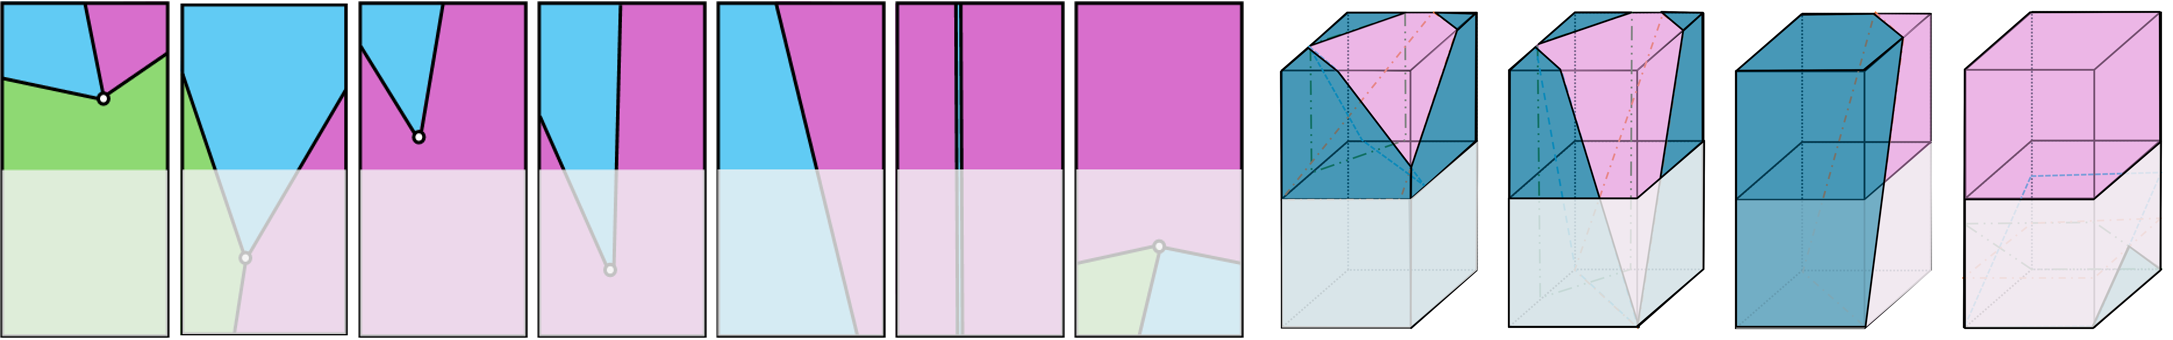
\includegraphics[width=\linewidth]{ext/fig_junction_full.png}
\caption{Junction schematics reproduced from~\cite{moeini2026foj3d}
(CC~BY~4.0). Left: 2D junctions with $M{=}3$ wedge regions. Right: 3D
junctions with $M{=}2$ regions formed by planes through a common vertex.}
\label{fig:junction}
\end{figure}

The full 3D FoJ objective couples all patches through a data-fidelity
term and two inter-patch consistency regularizers,
\begin{equation}
  \mathcal{L}(\theta)=\sum_p \Big[\underbrace{\|\hat y_p - y|_{\Omega_p}\|_2^2}_{\text{data}}
  + \lambda_B\,\mathcal{C}^{B}_p(\theta) + \lambda_C\,\mathcal{C}^{C}_p(\theta)\Big],
  \label{eq:loss}
\end{equation}
where $\mathcal{C}^B$ and $\mathcal{C}^C$ penalize disagreement between
each patch's local boundary and intensity maps and the global estimates.
Because every voxel belongs to multiple overlapping patches, the final
denoised volume is obtained by averaging all patch renderings covering
each voxel $x$:
\begin{equation}
  \hat x(x)=\frac{1}{|\{p: x\in\Omega_p\}|}\sum_{p:\,x\in\Omega_p}\hat y_p(x).
  \label{eq:avg}
\end{equation}

Optimization proceeds in two stages: $N_{\text{init}}$
\emph{initialization} iterations of discrete coordinate-descent search
over plane orientations and vertex positions, followed by $N_{\text{ref}}$
gradient-based \emph{refinement} iterations on Eq.~\eqref{eq:loss}.

%=====================================================================
\section{Results and Discussion}

We evaluate 3D FoJ across the three domains against identical classical
baselines: 3D Gaussian smoothing ($\sigma{=}1$), a $3^3$ median filter,
and 3D total-variation (TV)
denoising~\cite{rudin1992nonlinear,chambolle2004algorithm} swept over
weights $w\in\{0.05,0.1,0.2\}$. FoJ runs at its default schedule with
patch sizes $R\in\{6,8,12\}$ and stride $s{=}2$. In addition to 3D PSNR,
we measure a boundary F1-score on gradient-magnitude edge voxels to
quantify interface preservation.

\subsection{Reproducing the sparse-view CT ablation}

Before evaluating new domains, we reproduce the sparse-view CT ablation
of the original study (Table~3 of~\cite{moeini2026foj3d}), in which the
$256^3$ \emph{engine} volume is reconstructed from 20 cone-beam
projections corrupted by Poisson noise (``P50'') and then denoised with
3D FoJ at $R\in\{4,6,8,10,12\}$. The released repository contains the
FoJ model but not the CT simulation, view angles, or reconstruction
settings, so we rebuild the pipeline following the R$^2$-Gaussian
benchmark~\cite{zha2024r2gaussian} whose data generator the paper used:
TIGRE~\cite{biguri2016tigre} cone-beam geometry, 20 stratified-jitter
view angles in $[0,2\pi)$, and 60 CGLS iterations, followed by the
released FoJ implementation ($M{=}2$, stride 2).
Fig.~\ref{fig:teaser} shows the three low-SNR applications demonstrated
in the original study.

\begin{figure}[!hb]
\centering
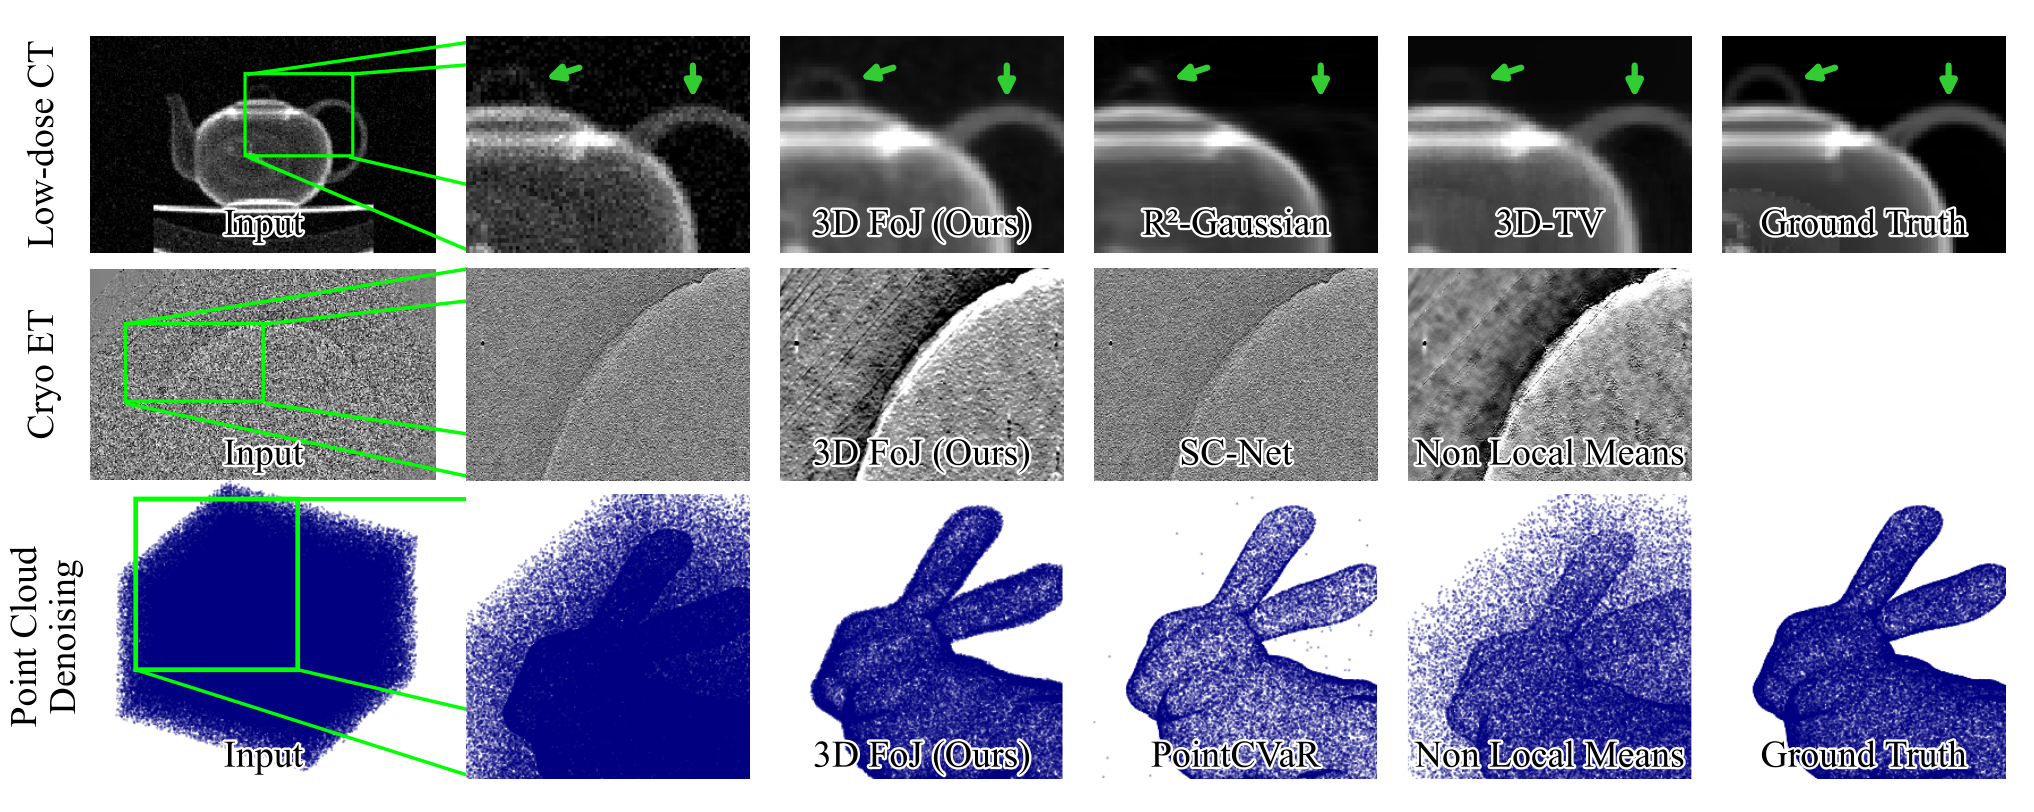
\includegraphics[width=0.85\linewidth]{ext/cvpr_teaser.png}
\caption{Figure 1 of the original paper, reproduced
from~\cite{moeini2026foj3d} (CC~BY~4.0): 3D FoJ applied to low-dose CT
(top row), cryo-ET (middle row), and point-cloud denoising (bottom
row).}
\label{fig:teaser}
\end{figure}

\begin{table}[!hb]
\centering\small
\begin{tabular}{lrrrrr}
\toprule
 & \multicolumn{5}{c}{$R$}\\
\cmidrule{2-6}
Metric & 4 & 6 & 8 & 10 & 12\\
\midrule
Reported PSNR          & 11.33 & 14.37 & 16.18 & 17.17 & 17.70\\
Ours PSNR              & 14.72 & 16.93 & 17.99 & 18.58 & \textbf{18.86}\\
$\Delta$ PSNR          & $+3.39$ & $+2.56$ & $+1.81$ & $+1.41$ & $+1.16$\\
\midrule
Reported MS-SSIM       & 0.762 & 0.784 & 0.796 & 0.798 & 0.800\\
Ours MS-SSIM           & 0.786 & 0.829 & 0.854 & 0.870 & \textbf{0.880}\\
$\Delta$ MS-SSIM       & $+0.024$ & $+0.045$ & $+0.058$ & $+0.072$ & $+0.080$\\
\bottomrule
\end{tabular}
\caption{Reproduction of the engine-volume CT ablation
of~\cite{moeini2026foj3d} (20 views, P50 Poisson noise). Ours uses the
released $M{=}2$ implementation on the unclamped CGLS-60 output;
$\Delta$ is ours minus reported.}
\label{tab:repro}
\end{table}

Table~\ref{tab:repro} compares the reported denoising quality with our
reproduction. The qualitative trend reproduces exactly: quality
increases monotonically with patch size, $R{=}12$ is best, and the
marginal gains shrink with each step ($+2.2$, $+1.1$, $+0.6$,
$+0.3\dB$). Our absolute PSNR sits $1.2$--$3.4\dB$ above the reported
values, consistent with the region count difference ($M{=}2$ in the
released code versus $M{=}3$ in the paper) and reconstruction details
the paper does not specify; the gap narrows with $R$ as the wedge
approximation becomes the dominant error. The released implementation
thus behaves as documented on the published benchmark, and the domain
study below uses it as-is.

\subsection{Porous-media micro-CT (Bentheim sandstone)}

We first test a $192^3$ central crop of Bentheim sandstone
micro-CT~\cite{bentheim2015zenodo} ($5.85\,\mu\mathrm{m}$ voxels,
normalized to $[0,1]$) under zero-mean additive Gaussian noise at
$\sigma\in\{15\%,30\%,40\%,55\%\}$ of the dynamic range. Because quartz
grains and pore spaces form near-constant phases spanning $10$--$35$
voxels separated by sharp interfaces, the volume satisfies both the
unbiased-input and patch-scale piecewise-flat requirements of Eq.~\eqref{eq:colors},
isolating the effect of the noise regime.

\begin{table}[H]
\centering\small
\begin{tabular}{lrrrrr}
\toprule
$\sigma$ & Noisy & Gaussian & Median & TV (best $w$) & FoJ (best $R$)\\
\midrule
15\% & 16.89 & \textbf{28.51} & 27.01 & 27.65 & 26.55\\
30\% & 12.00 & 25.26 & 22.26 & \textbf{26.03} & 25.64\\
40\% & 10.28 & 23.39 & 20.04 & 23.32 & \textbf{24.93}\\
55\% & \phantom{0}8.76 & 21.05 & 17.60 & 16.30 & \textbf{24.29}\\
\bottomrule
\end{tabular}
\caption{3D PSNR (dB) on Bentheim sandstone micro-CT. Classical filters
lead at moderate noise ($\sigma\le30\%$), whereas FoJ overtakes all
baselines once input PSNR drops below ${\sim}11$~dB ($\sigma\ge40\%$).}
\label{tab:bentheim}
\end{table}

Table~\ref{tab:bentheim} and Fig.~\ref{fig:curve} show the resulting
crossover. At $\sigma{=}15\%$ and $30\%$ (input PSNR $16.89$ and
$12.00\dB$), local statistics remain reliable enough for Gaussian and TV
filtering to recover the signal, and the coarse three-plane wedge
approximation introduces more bias than the noise it removes. Once the
input falls below ${\approx}11\dB$ PSNR ($\sigma{=}40\%$ and $55\%$),
classical filters either under-smooth the noise or blur across grain
boundaries, whereas averaging regional means over $R^3$ wedges
suppresses the variance while keeping planar interfaces intact. At
$\sigma{=}55\%$, FoJ exceeds the best classical baseline by $+3.24\dB$
and retains a boundary-F1 of $0.85$--$0.88$ compared with $0.54$ for TV
(Fig.~\ref{fig:slices}). Within this compatible regime, the optimal
patch size shifts from $R{=}6$ at $\sigma\le40\%$ to $R{=}8$ at
$\sigma{=}55\%$, before saturating at $R{=}12$ ($23.75\dB$) as patches
begin to exceed individual grain geometry.

\begin{figure}[!hb]
\centering
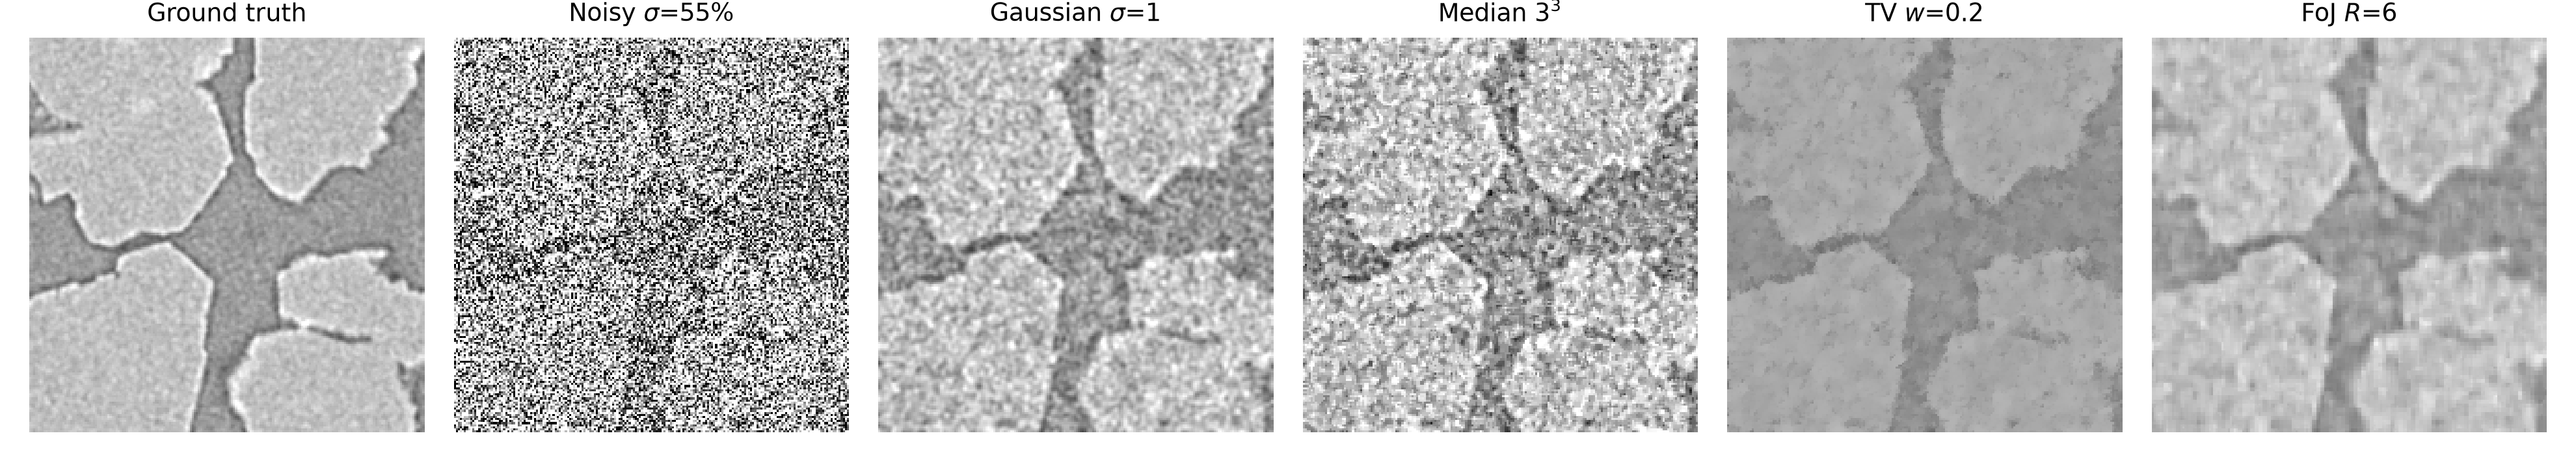
\includegraphics[width=0.85\linewidth]{fig_slices.png}
\caption{Bentheim micro-CT mid-slice at $\sigma{=}55\%$ Gaussian noise.
FoJ ($R{=}6$) preserves sharp grain--pore interfaces that Gaussian,
median, and TV filtering blur.}
\label{fig:slices}
\end{figure}

\begin{figure}[!hb]
\centering
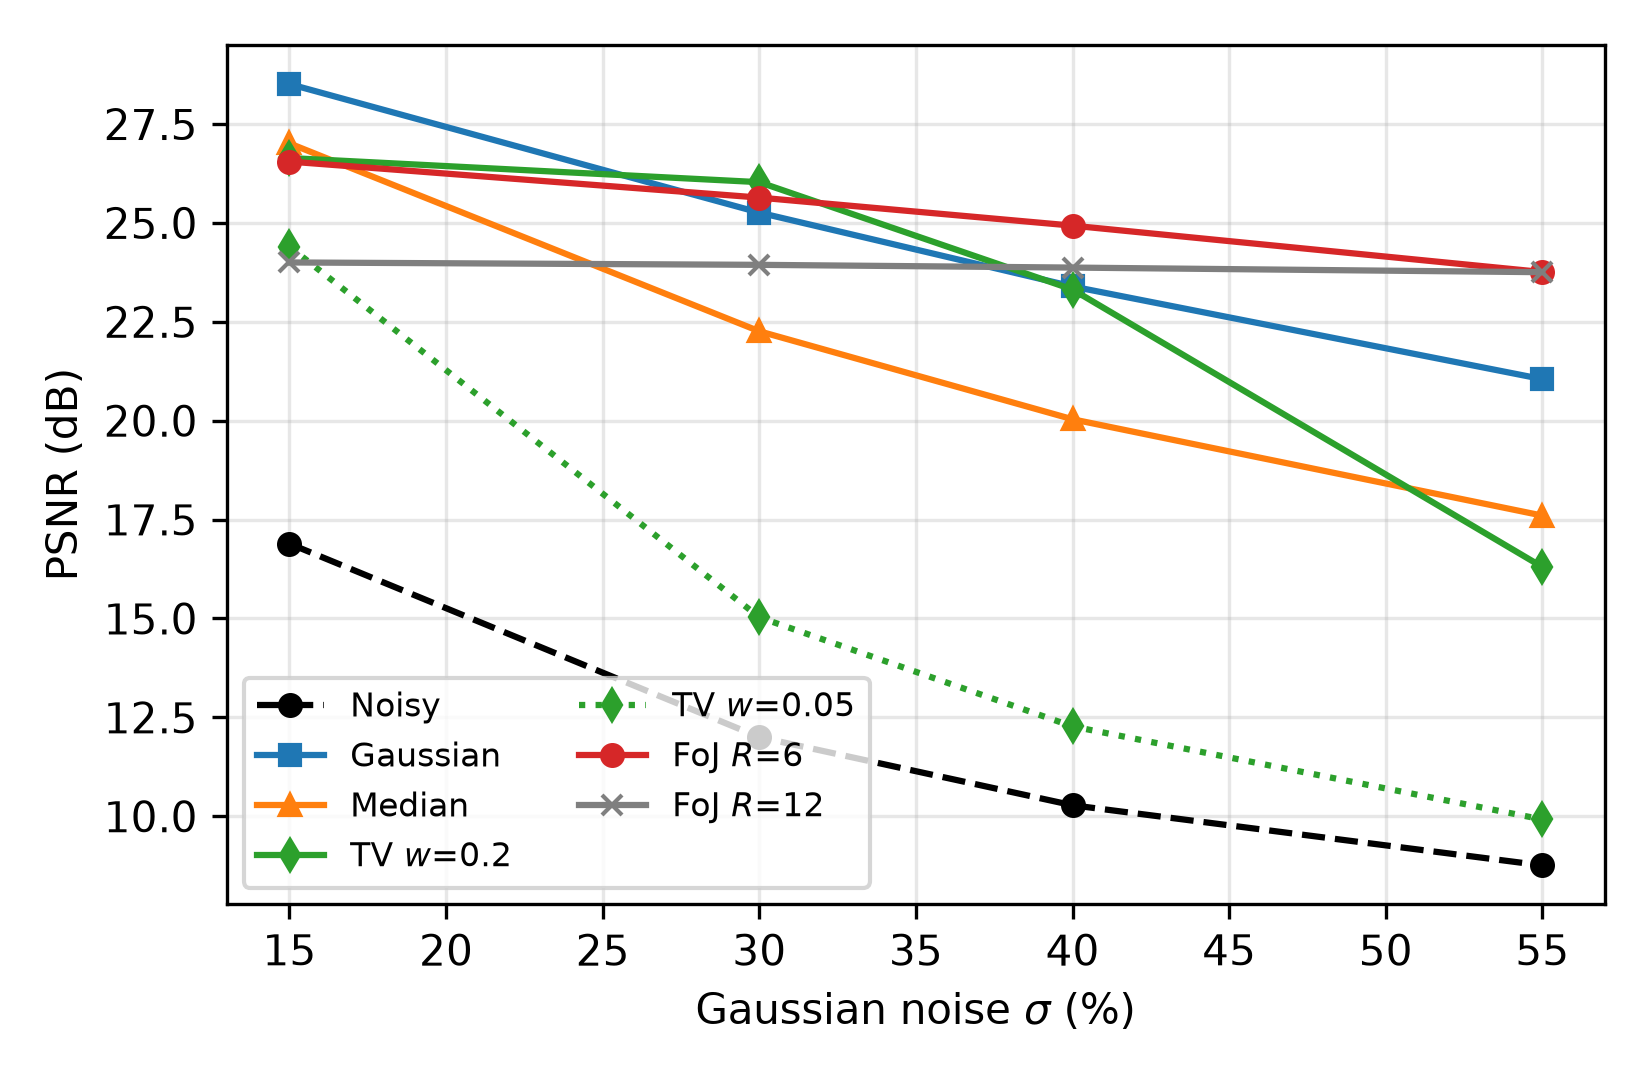
\includegraphics[width=0.48\linewidth]{fig_curve.png}
\caption{PSNR versus noise level on Bentheim micro-CT. FoJ (red)
overtakes the classical baselines between $\sigma{=}30\%$ and $40\%$.}
\label{fig:curve}
\end{figure}

\subsection{Volumetric MRI phantom (BrainWeb T1)}

To test what happens when structures are larger than the patch scale but
violate piecewise flatness, we evaluate the BrainWeb T1 brain
phantom~\cite{collins1998brainweb} ($181{\times}217{\times}181$, scaled
to $[0,1]$) under Rician noise at $\sigma\in\{3\%,5\%,7\%,9\%,13\%\}$.
Unlike porous rock, anatomical tissue exhibits smooth intensity
gradients within white and gray matter rather than flat plateaus.

\begin{table}[H]
\centering\small
\begin{tabular}{lrrrrrrr}
\toprule
$\sigma$ & Noisy & Gaussian & Median & TV (best $w$) & FoJ $R{=}6$ & FoJ $R{=}8$ & FoJ $R{=}12$\\
\midrule
3\%  & 29.19 & 28.69 & \textbf{30.80} & 29.85 & 25.67 & 24.02 & 21.56\\
5\%  & 24.69 & 26.10 & \textbf{27.25} & 26.62 & 24.14 & 22.66 & 20.59\\
7\%  & 21.74 & 23.80 & \textbf{24.58} & 24.00 & 22.52 & 21.43 & 19.78\\
9\%  & 19.55 & 21.87 & \textbf{22.48} & 21.94 & 20.99 & 20.19 & 18.88\\
13\% & 16.34 & 18.77 & \textbf{19.28} & 18.68 & 18.31 & 17.86 & 17.05\\
\bottomrule
\end{tabular}
\caption{3D PSNR (dB) on the BrainWeb T1 MRI phantom under Rician noise.
Because smooth tissue gradients cannot be represented by constant
wedges, FoJ trails classical filtering at every noise level and degrades
monotonically as patch size $R$ increases.}
\label{tab:mri}
\end{table}

As Table~\ref{tab:mri} shows, replacing each wedge with its regional
mean (Eq.~\eqref{eq:colors}) quantizes smooth tissue variations into
piecewise-constant steps. At $\sigma{=}3\%$, FoJ ($R{=}6$) reduces PSNR
below the noisy input itself ($25.67$ vs.\ $29.19\dB$) and trails the
$3^3$ median filter by $5.13\dB$. Although the gap narrows as noise
grows, reaching $0.97\dB$ at $\sigma{=}13\%$ as variance reduction
partially offsets model bias, FoJ never overtakes any classical
baseline, and larger patches ($R{=}8,12$) consistently perform worse
because they force constant values over wider tissue regions. Using FoJ
as a plug-and-play denoiser inside $4\times$-undersampled single-coil
MRI reconstruction shows the same limitation, reaching $27.99\dB$
compared with $30.39\dB$ for TV-PnP.

\subsection{Sub-patch binary porous media (sphere pack and Berea)}

Finally, we test two binary porous-media volumes, a synthetic sphere
pack and a segmented Berea sandstone scan~\cite{neumann2020sandstones}, under
additive Gaussian noise at $\sigma\in\{15\%,30\%\}$. Both volumes are
strictly piecewise-constant (binary solid and pore phases in $\{0,1\}$),
but their characteristic pore and grain features span only about
2~voxels, well below the smallest tested patch size ($R{=}6$).

\begin{table}[!hb]
\centering\small
\begin{tabular}{llrrrrrrr}
\toprule
Volume & $\sigma$ & Noisy & Gaussian & Median & TV (best $w$) & FoJ $R{=}6$ & FoJ $R{=}8$ & FoJ $R{=}12$\\
\midrule
Sphere pack & 15\% & 19.49 & 13.90 & 17.63 & \textbf{23.09} & 12.10 & 10.67 & 8.90\\
Sphere pack & 30\% & 13.48 & 13.77 & 15.52 & \textbf{17.82} & 12.04 & 10.65 & 8.89\\
Berea       & 15\% & \textbf{19.49} & \phantom{0}7.49 & \phantom{0}5.88 & 17.73 & \phantom{0}7.10 & \phantom{0}6.91 & 6.72\\
Berea       & 30\% & 13.48 & \phantom{0}7.45 & \phantom{0}6.37 & \textbf{13.61} & \phantom{0}7.09 & \phantom{0}6.91 & 6.72\\
\bottomrule
\end{tabular}
\caption{3D PSNR (dB) on binary porous-media volumes with ${\sim}2$-voxel
feature scale. Because sub-patch features cannot be partitioned by three
planes, each wedge mean collapses toward the global mean.}
\label{tab:binary}
\end{table}

Table~\ref{tab:binary} and Fig.~\ref{fig:collapse} show that when the
underlying geometry is finer than the patch support $\Omega_p$, the
wedge parameterization fails completely. Three planes through a single
vertex cannot separate dozens of 2-voxel pores inside an $R^3$ patch, so
every wedge covers a mixture of solid and pore voxels and
Eq.~\eqref{eq:colors} assigns each region an intensity near the patch
mean. Averaging overlapping patches in Eq.~\eqref{eq:avg} then produces
a nearly flat volume: on Berea at $\sigma{=}15\%$, the output standard
deviation drops from $0.49$ to $0.09$ and PSNR collapses from the noisy
input's $19.49\dB$ to $7.10\dB$ ($R{=}6$) and $6.72\dB$ ($R{=}12$).

\begin{figure}[H]
\centering
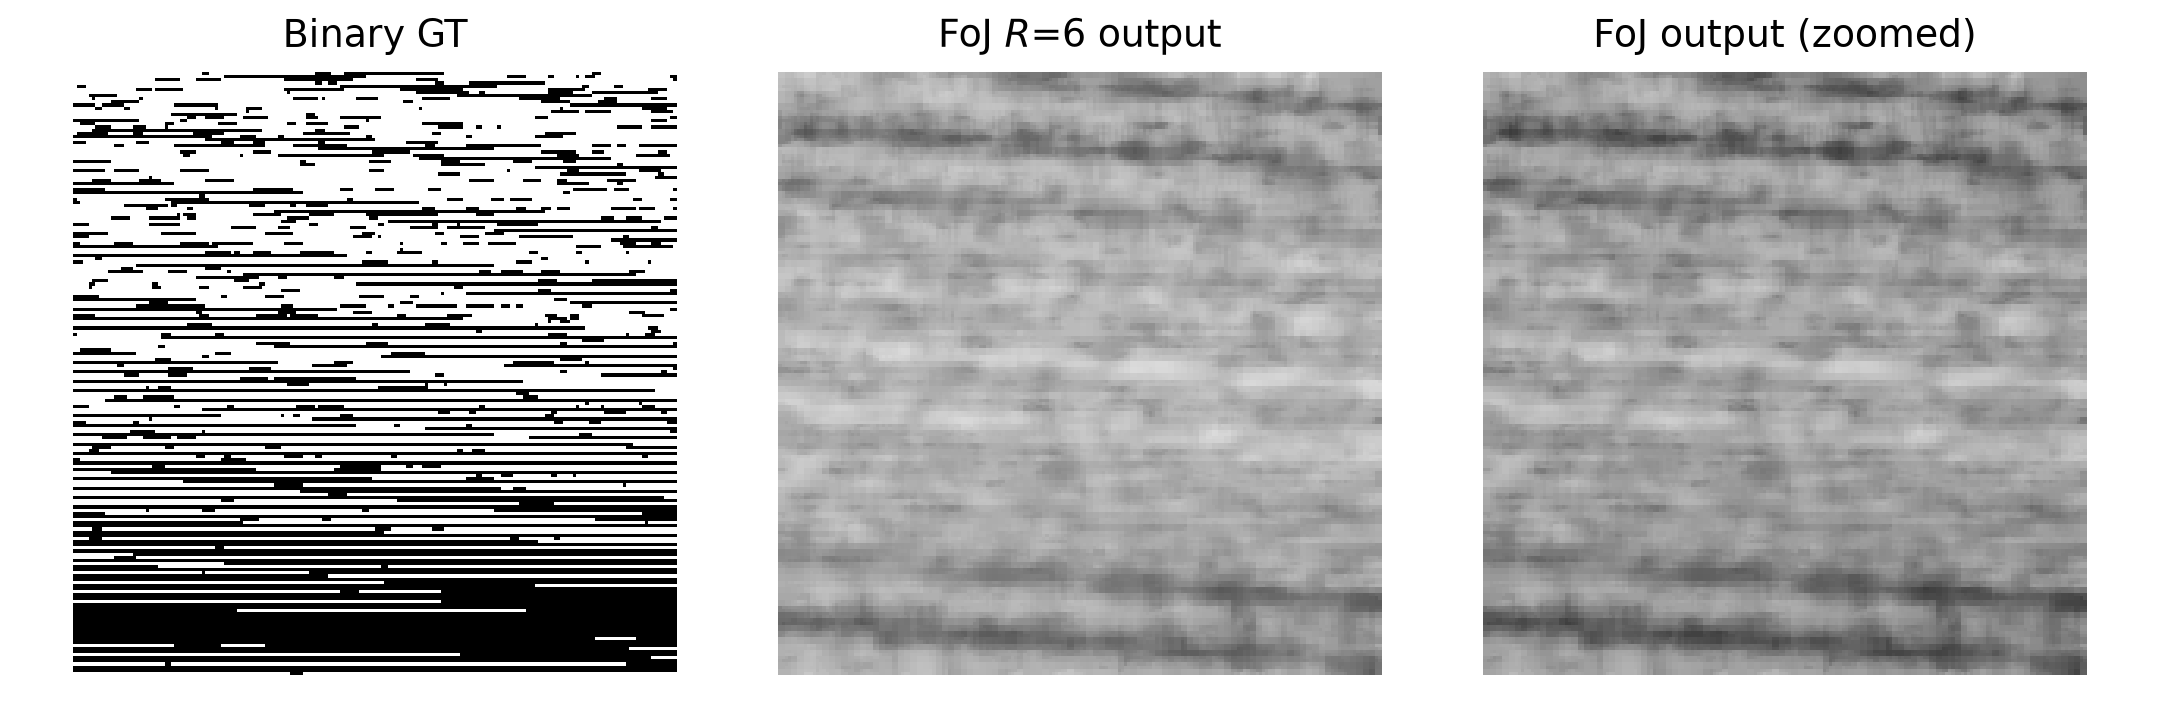
\includegraphics[width=0.55\linewidth]{fig_collapse.png}
\caption{Collapse on sub-patch-scale binary structure (Berea,
$\sigma{=}15\%$). Features of ${\sim}2$~voxels cannot be represented
inside $R{=}6$ patches, so regional means collapse the output toward the
volume mean.}
\label{fig:collapse}
\end{figure}

%=====================================================================
\section{Conclusion}

Evaluating 3D Field of Junctions across three volumetric domains outside
its original benchmark shows that its effectiveness is governed directly
by the regional-mean wedge formulation in Eqs.~\eqref{eq:colors}--\eqref{eq:avg}.
Because each patch is modeled as constant-valued wedges whose intensities
are local voxel means, any systematic offset in the input is preserved
rather than removed, and only structures that are piecewise-flat at or
above the patch scale $R$ can be represented. When the volume satisfies
these structural conditions, as in grayscale Bentheim sandstone
micro-CT where grains and pores span tens of voxels with sharp
interfaces, 3D FoJ overtakes Gaussian, median, and TV filtering once
the input PSNR falls below ${\approx}11\dB$, achieving a $+3.2\dB$
advantage and superior boundary retention at $\sigma{=}55\%$ because the
variance removed across each wedge outweighs the model's approximation
bias. Conversely, when the tissue is smooth (BrainWeb MRI), constant
wedges quantize real intensity gradients and underperform classical
filters at every tested noise level; when the features are smaller than
the patch (binary sphere pack and Berea sandstone), wedges cannot resolve
individual pores and the output collapses toward the global mean. 3D FoJ
is therefore a specialized, training-free prior for low-SNR volumes
whose phase structure is piecewise-flat and larger than the patch scale.

%=====================================================================
\begin{thebibliography}{99}

\bibitem{rudin1992nonlinear}
L.~I.~Rudin, S.~Osher, and E.~Fatemi.
\newblock Nonlinear total variation based noise removal algorithms.
\newblock \emph{Physica D}, 60(1--4):259--268, 1992.

\bibitem{chambolle2004algorithm}
A.~Chambolle.
\newblock An algorithm for total variation minimization and applications.
\newblock \emph{Journal of Mathematical Imaging and Vision}, 20(1):89--97,
2004.

\bibitem{buades2005nonlocal}
A.~Buades, B.~Coll, and J.-M.~Morel.
\newblock A non-local algorithm for image denoising.
\newblock In \emph{CVPR}, 2005.

\bibitem{dabov2007image}
K.~Dabov, A.~Foi, V.~Katkovnik, and K.~Egiazarian.
\newblock Image denoising by sparse 3-D transform-domain collaborative
filtering.
\newblock \emph{IEEE Transactions on Image Processing}, 16(8):2080--2095,
2007.

\bibitem{zhang2017beyond}
K.~Zhang, W.~Zuo, Y.~Chen, D.~Meng, and L.~Zhang.
\newblock Beyond a Gaussian denoiser: Residual learning of deep CNN for
image denoising.
\newblock \emph{IEEE Transactions on Image Processing}, 26(7):3142--3155,
2017.

\bibitem{verbin2021foj}
D.~Verbin and T.~Zickler.
\newblock Field of Junctions: Extracting boundary structure at low SNR.
\newblock In \emph{ICCV}, 2021.

\bibitem{moeini2026foj3d}
N.~Moeini, N.~Kim, J.~Romberg, and S.~Fridovich-Keil.
\newblock 3D Field of Junctions: A noise-robust, training-free structural prior
for volumetric inverse problems.
\newblock In \emph{ECCV}, 2026. arXiv:2603.02149.
\newblock Code: \url{https://github.com/voilalab/3D-Field-of-Junctions}.

\bibitem{zha2024r2gaussian}
R.~Zha, T.~J.~Lin, Y.~Cai, J.~Cao, Y.~Zhang, and H.~Li.
\newblock R$^2$-Gaussian: Rectifying radiative Gaussian splatting for
tomographic reconstruction.
\newblock In \emph{NeurIPS}, 2024.

\bibitem{biguri2016tigre}
A.~Biguri, M.~Dosanjh, S.~Hancock, and M.~Soleimani.
\newblock TIGRE: a MATLAB-GPU toolbox for CBCT image reconstruction.
\newblock \emph{Biomedical Physics \& Engineering Express}, 2(5):055010, 2016.

\bibitem{bentheim2015zenodo}
S.~Berg, H.~Ott, D.~Armstrong, A.~Schwing, J.~Humphrey, and R.~Necker.
\newblock High-resolution X-ray computed tomography images of Bentheim
sandstone (1~MPa, $5.854\,\mu\mathrm{m}$).
\newblock Zenodo, \url{https://doi.org/10.5281/zenodo.5548582}, 2021.

\bibitem{collins1998brainweb}
D.~L.~Collins, A.~P.~Zijdenbos, V.~Kollokian, J.~G.~Sled, N.~J.~Kabani,
C.~J.~Holmes, and A.~C.~Evans.
\newblock Design and construction of a realistic digital brain phantom.
\newblock \emph{IEEE Transactions on Medical Imaging}, 17(3):463--468, 1998.

\bibitem{neumann2020sandstones}
R.~Neumann, M.~Andreeta, and E.~Lucas-Oliveira.
\newblock 11 sandstones: raw, filtered and segmented data.
\newblock Digital Rocks Portal, \url{https://doi.org/10.17612/F4H1-W124}, 2020.

\end{thebibliography}

\end{document}
